\chapter{Installation \& User Guide}
In order to install the app 

1. enable access developer options and enable USB debugging
Instructions how to do that on Android device can be found here:

\url{https://www.howtogeek.com/129728/how-to-access-the-developer-options-menu-and-enable-usb-debugging-on-android-4.2/}

2. download APK at the following page:
\url{https://github.com/JoseIgnacioRetamalThomsen/FinalYearProject/tree/master/APK}

3. navigate to 'installation files' folder on your phone as illustrated in Fig.~\ref{fig:APK1}

4. change security settings by sliding (or checking) 'Unknown sources'

5. install the app by clicking 'install' button 

All the steps described above are illustrated in Fig.~\ref{fig:APK1}-Fig.~\ref{fig:APK6}

\begin{figure}[h!]
\begin{minipage}[t]{0.48\textwidth}
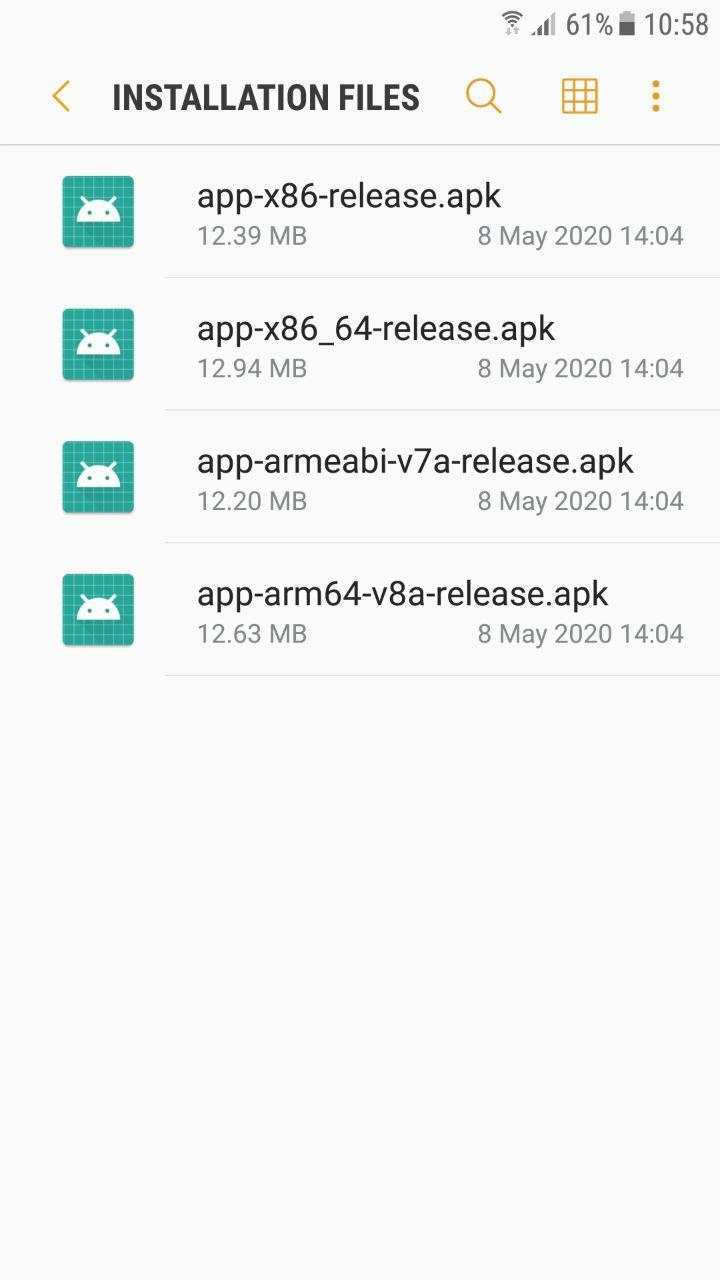
\includegraphics[width=\linewidth,keepaspectratio=true]{img/apk1.jpg}
\caption{APK1}
\label{fig:APK1}
\end{minipage}
\hspace*{\fill} % it's important not to leave blank lines before and after this command
\begin{minipage}[t]{0.48\textwidth}
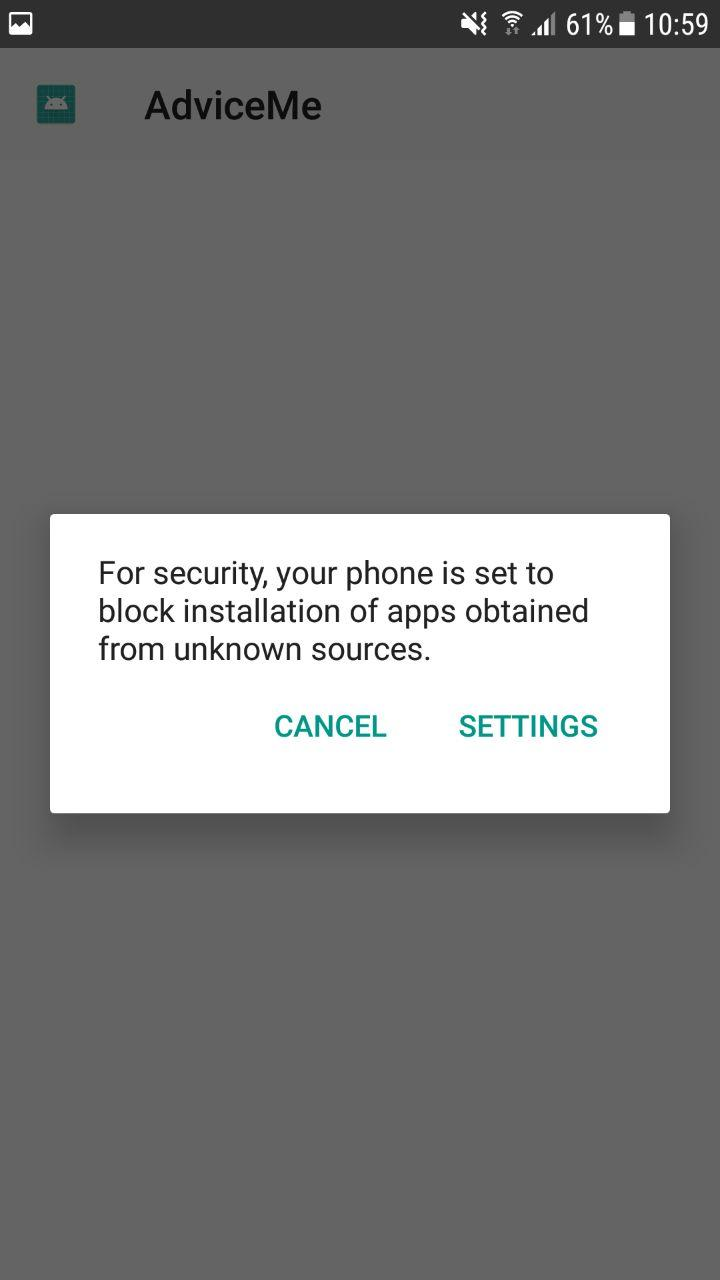
\includegraphics[width=\linewidth,keepaspectratio=true]{img/apk2.jpg}
\caption{APK2}
\label{fig:APK2}
\end{minipage}
\end{figure}

\begin{figure}[h!]
\begin{minipage}[t]{0.48\textwidth}
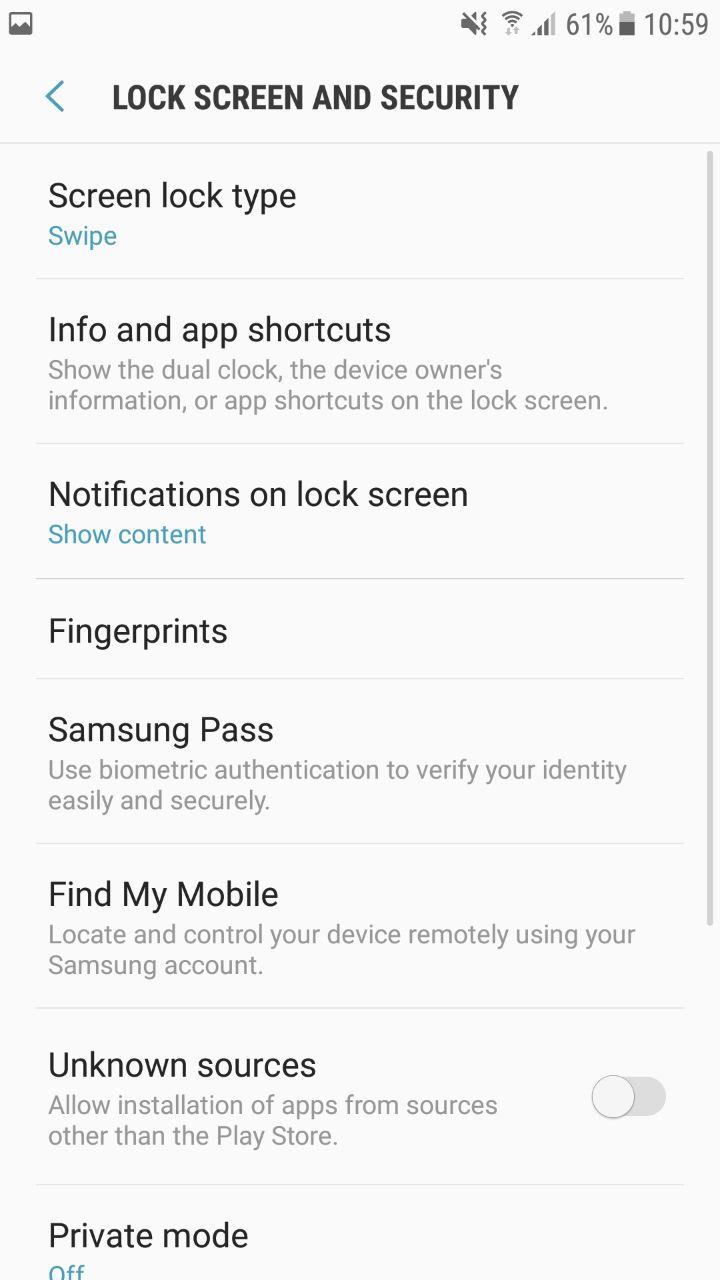
\includegraphics[width=\linewidth,keepaspectratio=true]{img/apk3.jpg}
\caption{APK3}
\label{fig:APK3}
\end{minipage}
\hspace*{\fill} % it's important not to leave blank lines before and after this command
\begin{minipage}[t]{0.48\textwidth}
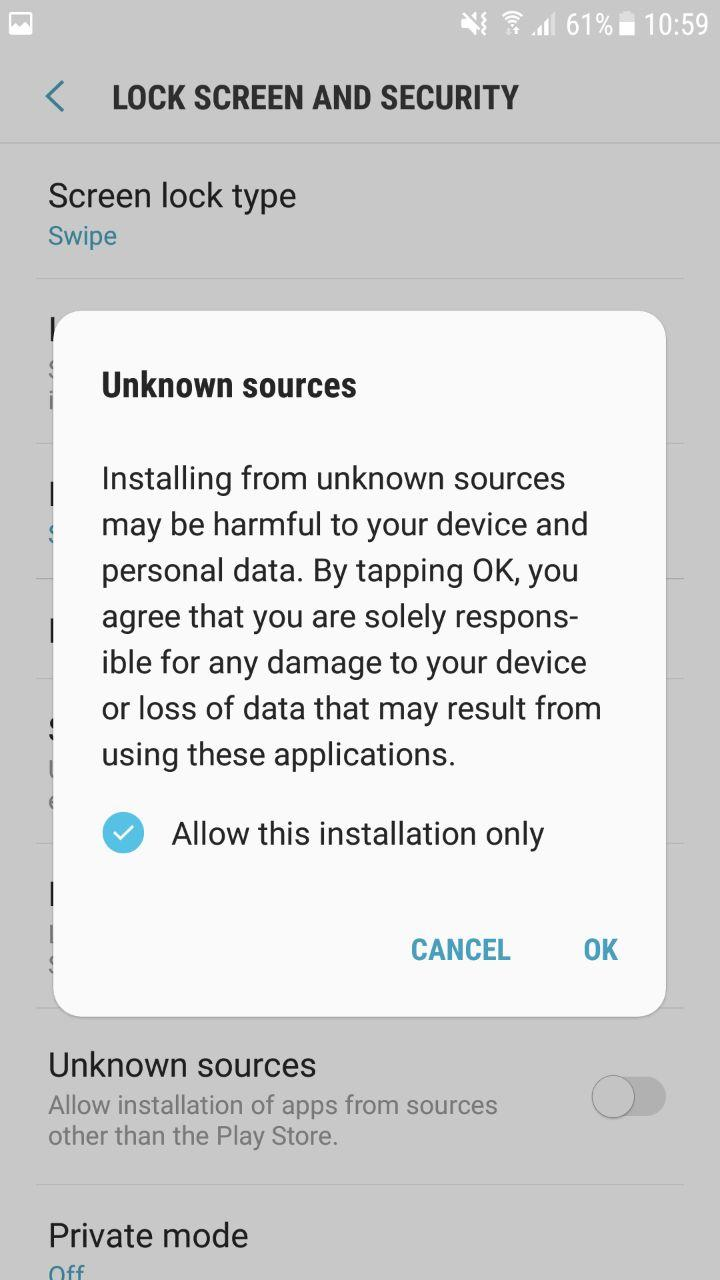
\includegraphics[width=\linewidth,keepaspectratio=true]{img/apk4.jpg}
\caption{APK4}
\label{fig:APK4}
\end{minipage}
\end{figure}


\begin{figure}[h!]
\begin{minipage}[t]{0.48\textwidth}
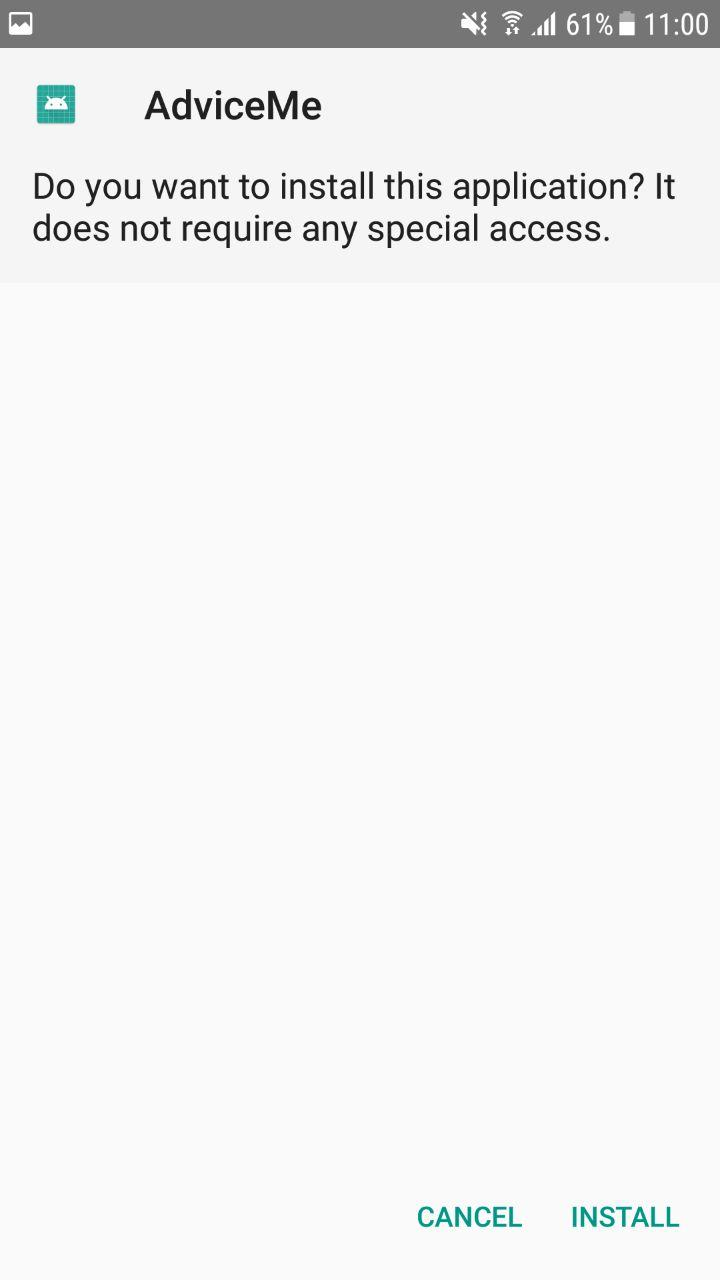
\includegraphics[width=\linewidth,keepaspectratio=true]{img/apk5.jpg}
\caption{APK5}
\label{fig:APK5}
\end{minipage}
\hspace*{\fill} % it's important not to leave blank lines before and after this command
\begin{minipage}[t]{0.48\textwidth}
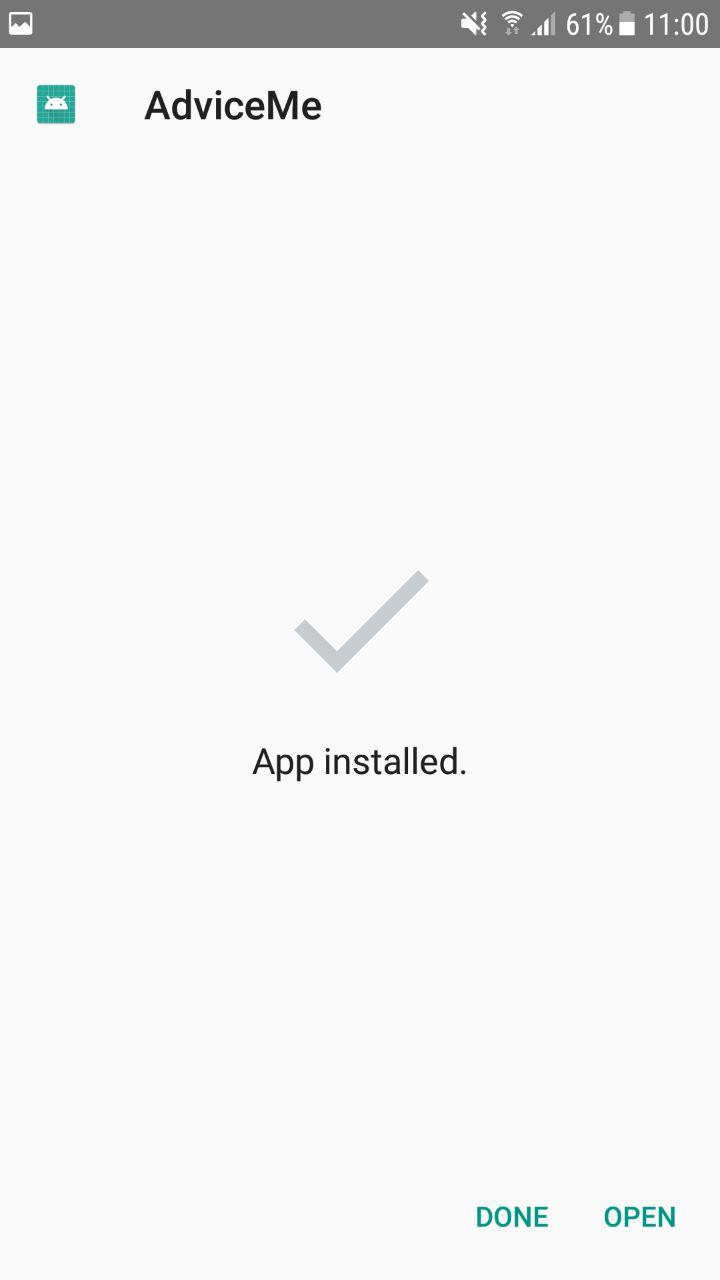
\includegraphics[width=\linewidth,keepaspectratio=true]{img/apk6.jpg}
\caption{APK6}
\label{fig:APK6}
\end{minipage}
\end{figure}

\

Video explaining how to use the app can be found at

\url{https://github.com/JoseIgnacioRetamalThomsen/FinalYearProject/tree/master/video}

